\documentclass[a4paper 12pt]{article}
\usepackage[margin=1in]{geometry}
\usepackage{natbib}
\usepackage{epsfig}
\usepackage{amsmath}
\usepackage{amsfonts}
\usepackage{float}
\usepackage{rotating} 
\usepackage{caption}
\usepackage{subfig}
\usepackage{booktabs}
\usepackage{adjustbox}
\usepackage[table]{xcolor}
\usepackage{tabularx}
\usepackage{caption}
\usepackage{enumerate}
\usepackage{enumitem}
\captionsetup{font=footnotesize}
\newcommand{\ra}[1]{\renewcommand{\arraystretch}{#1}}
\textheight 9.0 in
\textwidth 6.5 in
\topmargin -0.5 in
\oddsidemargin 0.0in
\renewcommand{\topfraction}{1}
\renewcommand{\bottomfraction}{1}
\renewcommand{\textfraction}{0}
\renewcommand{\floatpagefraction}{0.90}
\definecolor{TableEven}{rgb}{0.8000,0.9216,0.9490}
\usepackage{makecell}
%\usepackage{fourier} 
\numberwithin{equation}{section}
\usepackage{array}
\usepackage{titlesec}
\usepackage{sectsty}
\sectionfont{\centering}
\setcounter{secnumdepth}{4}
\usepackage{natbib}
\usepackage{siunitx}
\usepackage[toc,page]{appendix}
\usepackage{sectsty}
\usepackage{scalerel,stackengine}
\stackMath
\usepackage{graphicx}
%\titleformat{\subsection}    
%       {\normalfont\fontfamily{phv}\fontsize{12}{17}\bfseries\itshape}{\thesubsection}{1em}{}
\subsectionfont{\normalfont\bfseries\itshape}
\subsubsectionfont{\normalfont\itshape}
%\usepackage[colorlinks,citecolor=DeepPink4,linkcolor=DarkRed, urlcolor=DarkBlue]{hyperref}
%\usepackage[svgnames]{xcolor} 
%
%\usepackage[colorlinks]{hyperref}
%\hypersetup{citecolor=DeepPink4}
%\hypersetup{linkcolor=DarkRed}
%\hypersetup{urlcolor=DarkBlue}
%\usepackage{cleveref}

%hyperlink for website will need a better option. highlights all equations etc
 \usepackage{hyperref}


\renewcommand{\baselinestretch} {2.0}
\makeatletter
\setcounter{page}{1}
\def\doublespace{\def\baselinestretch{1}\@normalsize}
\def\enddoublespace{}
\title{\bf 
}   
% \footnotemark}
\author{}
\date{}
\@addtoreset{equation}{section}
\renewcommand{\sp}{\vspace{0.2 in}}
\renewcommand{\theequation} {\arabic{section}.\arabic{equation}}
%\renewcommand{\thefigure}{\arabic{section}.\arabic{figure}}
\renewcommand{\thefootnote}{\fnsymbol{footnote}}
\newtheorem{theorem}{Theorem}
\newtheorem{lemma}{Lemma}[section]
\newtheorem{remark}{Remark}[section]
\newtheorem{corollary}{Corollary}[section]
\newtheorem{exam}{Example}[section]
\newtheorem{proposition}{Proposition}[section]

\newcommand{\Bigskip}{\vspace{0.3 in}}

\usepackage{xspace}
\newcommand{\m}{\textnormal{\sffamily m}\xspace}
\newcommand{\cm}{\textnormal{\sffamily cm}\xspace}
\newcommand{\g}{\textnormal{\sffamily g}\xspace}
\newcommand{\kg}{\textnormal{\sffamily kg}\xspace}
\newcommand{\SE}{\textnormal{\sffamily SE}\xspace}
\newcommand{\RSE}{\textnormal{\sffamily RSE}\xspace}
\newcommand{\LB}{\textnormal{\sffamily LB}\xspace}
\newcommand{\UB}{\textnormal{\sffamily UB}\xspace}

% command for commenting
\usepackage{color}
\usepackage{ulem}
\newcommand{\ed}[1]{\textcolor{red}{#1}}
\newcommand{\nat}[1]{\textcolor{blue}{#1}}
\definecolor{darkgreen}{rgb}{0.09, 0.45, 0.27}
\newcommand{\olav}[1]{\textcolor{darkgreen}{#1}}

\makeatletter
\let\latex@xfloat=\@xfloat
\def\@xfloat #1[#2]{%
  \latex@xfloat #1[#2]%
  \def\baselinestretch{1}
  \@normalsize\normalsize
  \normalsize
}
\makeatother

\newcommand\longitude[1]{\directlua{ longitude ( \luastring{#1} ) }}


\usepackage{lineno}
\linenumbers

 
\begin{document}
%\title{Optimising sampling effort of the North Sea International Bottom Trawl Survey Data}


\title{An analysis of the North Sea International Bottom Trawl Survey Data}

\maketitle


\begin{abstract}

In this research we present estimation procedures for calculating abundance at age indices, and investigate the sensitivity of these indices with respect to the number of otoliths collected at sea. The procedures presented are applied to the North Sea International Bottom Trawls Survey data for cod (\textit{Gadus morhua}) and saithe (\textit{Pollachius virens}). We demonstrate how much information would be lost if the survey design was defined such that fewer otoliths were collected. Age length keys (ALKs) are used to map lengths to age, and we use ALKs with and without the assumption of constant age length structures over relatively large areas. All abundance at age indices are presented with variance estimates. \\
%In this research we present an approach for optimising sampling effort of the North Sea International Bottom Trawl Survey Data. 

\end{abstract}

\section{Plan}
\begin{itemize}

\item Olav: 
\begin{enumerate}

	\item Implement sampling procedure such that we sample 1. Hauls, 2. Remove ages, 3. Calculate mCPUE 
\item 	Change the removal procedure such that otoliths are kept with probability proportional to the number of fish measured with the corresponding cm group.
\item Include the uncertainty in the ALK in the model.
\item Change the ALK procedure such that the grouped length groups are directly used in the ALK. That is construct a common ALK for every cm in the cm group.
\item length stratification is done for two reasons: 1) make sure all length groups are covered as the catches may be different (e.g., fewer older fishes may be caught), 2) correct for selection bias (as random sampling is difficult. size sorting could be problematic so length- stratifying helps to address this problem. Keep a stratification regime that is sub-optimal. Proportional sampling we expect higher uncertainty for older fishes when length classes are merged, e.g., 1 otolith per 5cm. Many younger fishes and fewer older fishes so probability of selection of older fishes is lower compared with the younger fish, even if we can go to very large length groups e.g, 7 cm without sacrificing the precision, but it would be bias estimates). So important to decide on maximum length group
\end{enumerate}
\item Natoya

\begin{enumerate}
\item Edit paper uptil the removal procedure.
\item	If time: Create a function which given a haul id, species and length returns the number of fish caught with that length in that haul of that species. This is needed in point 2 in Olav’s list.

\end{enumerate}
\end{itemize}

\section{Bootstrap procedure by \citet{aanes2015efficient}}
We used nonparametric bootstrapping (Efron 1982) to estimate the variance of age compositions and proportions-at-age for all estimators. The bootstrap resampling procedure replicated the multistage sampling designs. Since the sampling fraction of PSUs generally is negligible, we assumed sampling with replacement in the first stage (see, e.g., Williams 2000). Each bootstrap replicate was generated by first sampling the PSUs at random with replacement. The age samples within each PSU were then selected by simple random sampling (catch data) or by systematic sampling from length bins (stratified sampling; trawl survey data). Since the age samples generally were collected from a relatively small finite population of fish measured for length, the bootstrap subsamples
within PSUS were selected without replacement, using methods described in Booth et al. (1994) and Davison and Hinkley (1997). The effect of subsampling sizes on the precision of age compositions was studied through simulations, where we varied the number of age samples from each PSU in the bootstrap resampling. The bootstrap estimates of variance for each survey were based on 2000 replicates.


\section{Methods}

\subsection{Catch per unit effort}
\label{sec:cpueestimators}
In this research, the catch per unit effort (CPUE) is defined as the number of fish of a certain species and age or length which are caught per hour trawl. In this section we define the CPUE mathematically, which explains how the index is calculated. For a given species of interest, let $n_{h,l}$ be the number of fish with length $l$ caught by trawl haul $h$. The CPUE for a given length $l$ by trawl haul $h$ is defined as 
\begin{equation}\label{eq:cpueHaul}
\mathrm{CPUE}_{h,l} =\frac{n_{h,l}}{d_h},
\end{equation}
were $d_h$ is the duration of the trawl in hours. The CPUE per age class is further defined as
\begin{equation}\label{eq:cpueALK}
\mathrm{CPUE}_{h,a} =\sum_{l \in {\bf L}}\mathrm{CPUE}_{h, l} \times ALK_{a,l,h},
\end{equation}
where ${\bf L}$ is the set of all length classes and $ALK_{a,l,h}$ is the age length key, which represents the estimated proportion of fish with age $a$ in $l$th length class in haul $h$. For a given number of trawl hauls in a statistical rectangle, the mean CPUE defined as  mCPUE  in a statistical rectangle can be expressed as the average CPUE of the trawl hauls in the statistical rectangle:
\begin{equation}\label{eq:cpueRec}
\mathrm{mCPUE}_{s,a} =\sum_{h \in H_{s}}\frac{\mathrm{CPUE}_{h,a}}{|H_{s}|}.
\end{equation}
Here $H_{s}$ represents the set of trawl hauls taken in statistical rectangle $s$, and $|H_{s}|$ is the number of hauls taken in the rectangle. The mCPUE in $p$th RFA is further defined as
\begin{equation}\label{eq:cpueRFA}
\mathrm{mCPUE}_{p,a} = \sum_{s \in S_{p}} \frac{\mathrm{mCPUE}_{s,a}}{|S_{p}|} \omega_s,
\end{equation}
where $S_{p}$ is the set of all statistical rectangles in RFA $p$, $|S_{p}|$ is the number of statistical rectangles in RFA $p$, and $\omega_s$ is a weight variable for each statistical rectangle. The weight variable $\omega_s$ varies between species. For some species $\omega$ equals 1 (e.g. Gadus morhua) for all $s$, and for other species it is the proportion of the statistical rectangle which has depth between 10 to 200 meters, for example Pollachius virens (see Table \ref{tab:weights} in Supplementary Materials \ref{secAp:weightings}).  The mean catch per unit at age in the whole study area, $\lambda_{a}$, is defined by
\begin{equation}
\lambda_{a}= \frac{\sum_{p\in {\bf P}} A_{p}  \mathrm{mCPUE}_{p,a}}{A_{\text{total}}}.
\label{abundanceestimatornorthsea}
\end{equation}
This is know as the index of abundance at age, where ${\bf P}$ is the set of RFAs, $A_p$ is the area of RFA $p$, and $A_{\text{total}} = \sum_{p\in {\bf P}} A_{p}$.
%mCPUE_{N,a} 


\subsection{ALK estimators}
\label{sec:alkmethods}
The definition of the CPUE of age includes an ALK, see (\ref{eq:cpueALK}), which we described in this section. Three ALK estimators are included in this research, which are named as follows:  \textit{i}) DATRAS ALK, \textit{ii}) haul based ALK and \textit{iii}) model based ALK.
% In this section we define these three ALK estimators. 
\subsubsection{DATRAS ALK}
\label{sec:datrasalkestimator}
Let $\text{ALK}^{\text{D}}$ denote the ALK used in DATRAS to estimate abundance at age for the IBTS data. The $\text{ALK}^{\text{D}}$ is defined as constant within each RFA, and is calculated for each RFA by aggregating the age observation from each RFA. $ALK^{\text{D}}_{a,l,h}$ used in equation (\ref{eq:cpueALK}) is defined as the proportion of observed fish with age $a$ in length class $l$ in the RFA $h$. If there are no observed fish in length class $l$ in the RFA, ages from length classes close to $l$ is used. The details of the procedure for borrowing strength from neighbouring length classes are given in Supplementary Materials \ref{secAp:DATRASBorrow}. The underlying assumption of this ALK  is that age-length compositions are homogeneous within the RFAs. This is a rather strong assumption, and any violation would have an unknown impact on the estimates of abundance indices. \citet{aanes2015efficient} illustrated that violation of the assumption of constant ALK leads to biased estimates of CPUEs. 

\subsubsection{Haul based ALK}
\label{sec:haulestimator}
We define a haul dependent ALK  by  $ALK^{H}$. The $ALK^{H}_{a,l,h}$  used in equation (\ref{eq:cpueALK}) is defined as the average proportion of observed fish with age $a$ in  length class $l$ in haul $h$. If there are no observed ages of fish in a length class $l$ in the haul, ages from the same length class in the haul close by is used (see Supplementary Materials \ref{secAp:oursBorrow} for the procedure).

\subsubsection{Model based ALK}
\label{sec:spatialModelALK}
In this section we introduce a spatial model based ALK, which we define as $\mathrm{ALK^M}$. Using such a model enables us to obtain smooth structures in the distribution of age given length. It further enables us to utilize spatial latent effects. Spatial model based approach of age-lengths are widely used \citep{berg2012spatial, hirst2012bayesian, rindorf2001analyses}, and are used for stock assessment in the North Sea \citep{berg2014evaluation}.  % kvist2000using olav: double check this when i have access.

Let the response variable of the age group of a fish be $a = M,...,A$ where $M$ is the youngest age, and $A$ is the oldest age which is typically defined as a "plus group". Suppose $y(l,{\bf s})$ is the age  of a fish with length $l$ caught at location ${\bf s}$. As in \citet{berg2012spatial} we use a continuous ratio model for the spatial age given length model. However, in our application we assume for each species we know a length $l^*$ such that all fish above length $l^*$ are above age $M$, and all fish with length below $l^*$ are of age below $A$. By including such a variable we reduce the number of parameters in the model by removing one linear predictor. Define the continuous ratio we are modelling as
\begin{equation}\label{eq:linearPred1}
\pi_a[y(l,{\bf s})] = \frac{p_a(l,{\bf s})}{p_a(l,{\bf s}) + \cdots + p_{A}(l,{\bf s}) +p_{M}(l,{\bf s}) } \vspace{ 4mm} \ \ \ \text{for } a =M+1,...,A-1 ,
\end{equation}
where \vspace{-5mm} $p_a(l,s)$ is the probability of a fish with length $l$ at location ${\bf s}$  to be of age $a$.  Note  that either $p_{A}(l,{\bf s})$ or $p_{M}(l,{\bf s})$ is known to be equal to zero, and the other is selected such that $\sum_a p_a = 1$. We further assume the logit link
\begin{equation}\label{eq:linearPred}
\log \left[ \frac{\pi_a[y(l,{\bf s})]}{1-\pi_a[y(l,{\bf s})]}\right] = f_a(l) + \gamma_a({\bf s}).
\end{equation}
Here $ f_a(l)$ is a continuous function of length and $\pmb{\gamma}$ is a mean zero Gaussian spatial random field with Mat\'{e}rn covariance function \olav{\citep{stein2012interpolation}}. The spline $f_a$ is intended to account for that longer fish are typically older, and the spatial random field, $\pmb{\gamma}$, is intended to account for spatial variation in the ALK (see Table \ref{tab:parameters} for a description of the parameters used in (\ref{eq:linearPred})). 

The continuous function $f_a(l)$ in (\ref{eq:linearPred}) is modelled with usage of P-splines \citep{wood2017generalized}, and these spline regression coefficients are included as a Gaussian random effect. The precision matrix for the spline regression coefficients is constructed such that the variability (or wryggliness) in the spline is penalized, see \citet[page 239]{wood2017generalized} for details. The R package mgcv \citep{wood2015package} is used for extracting the precision matrix needed for the spline regression coefficients. The marginal variance of the P-splines regression coefficients, $\sigma_f^2$, is estimated in our inference procedure. 

We assume that the spatially Gaussian random field in (\ref{eq:linearPred}), $\pmb{\gamma}$, follows a stationary Mat\'{e}rn covariance structure:
\begin{equation}\label{eq:matern}
 \text{Cov}(\gamma(\mathbf{s}_1),\gamma(\mathbf{s}_2)) = \frac{\sigma^2_{\gamma}}{2^{\nu-1}\Gamma(\nu)}(\kappa||\mathbf{s}_1 -\mathbf{s}_2||)^{\nu}K_{\nu}(\kappa||\mathbf{s}_1-\mathbf{s}_2||),
\end{equation}
where $\sigma^2_{\gamma}$ is the marginal variance, $||\mathbf{s}_1-\mathbf{s}_2||$ is the distance between $\mathbf{s}_1$ and $\mathbf{s}_2$ in kilometres, $\kappa$ is a spatial scale parameter, $\nu$ is a smoothing parameter and $K_{\nu}(\cdot)$ is the modified Bessel function of the second kind with $\nu = 1$.  The spatial field is estimated with the stochastic partial differential equation (SPDE) procedure described in \citet{lindgren2011explicit}. The main concept behind the SPDE procedure is that the precision matrix of a spatial field with Mat\'{e}rn  covariance function can be approximated by a sparse matrix on a grid covering the area of interest. Such a grid and sparse precision matrix are constructed with use of the R-INLA package \citep{rue2009approximate}. See figure \ref{fig:mesh} for an illustration of the mesh used in the case study for cod.


\begin{figure}[h!]
\begin{center}
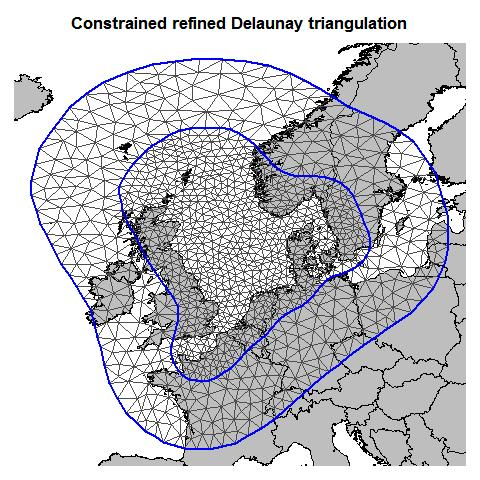
\includegraphics[scale=0.5]{figures/mesh.jpeg}
 \caption{Mesh used in the case study for cod in section \ref{sec:data} for approximating (\ref{eq:matern}) with the SPDE-procedure.}\label{fig:mesh}
\end{center}
\end{figure}


The species specific constant $l^*$ is selected as the mid point between the shortest fish of age A and the longest fish of age M in the corresponding year and quarter. A sensitivity analysis of this constant is performed by adjusting it up and down 5 cm for cod in year 2018 in Q1. The point estimate of the mCPUEs then changed in the forth decimal, which we consider to be negligible.

The model based ALK estimate is obtained by maximizing the likelihood. We maximize the likelihood with use of an R-Package called Template Model Building {\sffamily TMB} \citep{kristensen2015tmb}, combined with the optimizing function {\sffamily nlminb} in R. In this application {\sffamily TMB} is advantageous as it uses Laplace approximation for the latent fields gaining computational efficiency, it also utilizes sparse structures in the latent fields, and uses automatic derivation. \\

\begin{table}[hh!]
\begin{tabular}{lllllr}
Parameter &\bf{Explanation}  \\
\midrule
$\sigma_f^2$	& Marginal variance of the spline regression coefficients \\
$\sigma_{\gamma}^2$ &Marginal variance of the spatial field in (\ref{eq:matern})			\\
$\kappa$	&  Spatial scale parameter of the spatial field	in (\ref{eq:matern})\\
\bottomrule
\end{tabular}
\caption{\textit{The three parameters used in the ALK model.}}
\label{tab:parameters}
\end{table}


\subsection{Uncertainty estimation}
\label{sec:uncertaintyestimation}
In this section we describe how the uncertainty of the CPUE estimates are calculated. We use nonparametric bootstrapping to quantify the uncertainty of the CPUEs. In nonparametric bootstrapping independent samples of lengths and age are drawn with replacement from the original data and approximate $95\%$ confidence intervals are obtained using bias-corrected percentile method  \citep{carpenter2000bootstrap}. Nonparametric resampling allows us to estimate the sampling distribution of the CPUE empirically without making assumptions concerning the data. The bias-Corrected method adjusts for the bias and skew of the sampling distribution of the data \citep{puth2015variety, karlsson2009bootstrap}. The bootstrap procedure is given in Supplementary Materials \ref{secAP:nonparametricbootstrap}.  

A bootstrap procedure for estimating the uncertainty of CPUEs in the North Sea is suggested in \nat{\citet{ICES2006Report}}. This procedure is given in Supplementary Materials \ref{secAP:nonparametricbootstrap}. In the rest of this research, we refer to this procedure as DATRAS bootstrap procedure. This procedure is outlined in DATRAS for uncertainty estimation of IBTS indices but so far it has not been implemented.  The DATRAS procedure is divided into two parts; one part which samples CPUE per length (\ref{eq:cpueHaul}), and another part which samples the ALK used in (\ref{eq:cpueALK}). The DATRAS bootstrap procedure is based on the assumption of homogeneous CPUE within RFAs. This assumption is likely to be wrong, and would typically cause an overestimation of the uncertainty.  Therefore, we have included a bootstrap procedure, defined as the stratified bootstrap procedure, which instead assumes constant CPUE within each statistical rectangle. 

\subsubsection{DATRAS and Stratified bootstrap procedure}
\label{sec:datrasstratifiedbootstrap}
In this section we describe the bootstrap procedure for catch at length proposed in \emph{DATRAS} \citet{ICES2006Report} and the stratified procedure, and elaborate how the ALK is simulated. Assume there are $N_{\text{s}}$ trawl hauls in a statistical rectangle. The DATRAS bootstrap procedure consists of sampling with replacement $N_{\text{s}}$ of all trawl hauls in the corresponding RFA, and place them in the statistical rectangle. This procedure is performed independently across all statistical rectangles. It should be remembered that this procedure is based on the assumption that ALK is homogeneous in the whole RFA, and the implication of DATRAS bootstrap procedure on indices of abundance is two-fold. Firstly, DATRAS bootstrap procedure ignores the fine-scale stratification in the sampling process. This would lead to an overestimation of the uncertainty. Secondly, it ignores the sampling procedure of age-length data collected at the haul level. This would lead  to an underestimation of the uncertainty. So there are biases in both directions, which are difficult to quantify. The Stratified bootstrap procedure is a modification of the DATRAS bootstrap procedure. Rather than sampling hauls from the whole RFA, we  sample the $N_{\text{s}}$ trawl hauls from the list of hauls within the same statistical rectangle. If there is only one trawl haul within a statistical rectangle, we sample either that haul or the closest haul.

To estimate the ALK used in DATRAS ($\mathrm{ALK}^{D}$) we sample with replacement age observations within each RFA stratified with respect to length. If there is only one observed age from a given length class, we sample either that age or, at random, an age of the closest length class with observed ages. For both the haul based ALK and the model based ALK, we use the ages in the sampled hauls obtained when simulating the CPUE per length.

%\ed{(Are we not missing a description of the ALK-bootstrap for haul-based and model based, and a description of how the bootstrap of hauls is integrated with the bootstrap of ALKs (the nested bootstrap loop) ?)} 


\bibliographystyle{apalike}
\bibliography{ibtsBib}
\end{document}